\documentclass[times, utf8, seminar]{fit}

%\batchmode
%\usepackage{booktabs}
\usepackage{listings}
\usepackage{longtable}
\usepackage{xcolor}
\usepackage{float}
\usepackage{enumitem}
\usepackage{hyperref}
\usepackage{enumerate}
\usepackage{graphicx}
\usepackage{etoolbox}
\usepackage{datetime}
\usepackage{needspace}
\usepackage{titlesec}
%\usepackage{hyperref}
%\titleformat{\chapter}[display]{\normalfont\huge\bfseries}{\chaptertitlename\ \thechapter}{20pt}{\Huge}

\begin{document}
\widowpenalty=300
\clubpenalty=300

\lstset{
  language=bash,
  backgroundcolor=\color{gray!25},
  basicstyle=\ttfamily \footnotesize,
  breaklines=true,
  prebreak=\raisebox{0ex}[0ex][0ex] \hookleftarrow,
  columns=fullflexible
}


% this alters "before" spacing (the second length argument) to 0
%\titlespacing*{\chapter}{0pt}{0pt}{40pt}

% this changes "before" spacing back to its default of 50pt
%\titlespacing*{\chapter}{0pt}{50pt}{40pt}}

%\titlespacing*{\chapter}{0pt}{-50pt}{18pt}
%\titleformat{\chapter}[display]{\normalfont\huge\bfseries}{\chaptertitlename\ \thechapter}{20pt}{\Huge}

\title{Agilni \em{software development},\newline GIT SCM}

\author{Ernad Husremović}
\brindex{DL 2792}
\verzija {0.0.1}

\mentor{mr. Adil Joldić}

\maketitle

\tableofcontents

%\listoftables
%\listoffigures
\newpage

\begin{abstract}

Dokument na bazi konkretnog primjera\footnote{"HOWTO" stil} objašnjava uobičajeni developerski `workflow' pri korištenju GIT `Source Code Management' (SCM) alata. 
U primjeru se koriste GIT web servisi `Github'\footnote{\url{https://www.github.com}} i `Gitlab'\footnote{\url{https://gitlab.knowhow.out.ba}, \url{http://gitlabhq.com}}.
Čitalac će upoznati osnovne operacije GIT klijenta i način korištenje navedenih web servisa.


\keywords{open source software, OSS, Source code management, SCM, DSCM, Version control, GIT}
\end{abstract}

% abstract end

\chapter{Uvod}
\vspace*{-0.7cm}

\section{`Source code management' (SCM) software}

`Source code management' (SCM) software obezbjeđuje pohranu različitih verzija programskog koda u zajednički repozitorij. 
Iako je prvobitna ovih alata bilo čuvanje programskog koda, oni se mogu koriste za za pohranu (verzioniranje) svih artifakta softverskog projekta uključujući dokumentaciju, dijagrame, binarni kod.
Ovaj software se često naziva i `Version control' software.

Sa stanovišta arhitekture, SCM sistemi se dijele na centralizovane i distribuirane (DSCM).

\subsection{Centralizirani (mrežni) SCM}

Najpoznatiji predstavnici su `CVS' i `Subversion'. `CVS' je među prvim SCM alatima-ima koji je postigao veliku popularnost.

`Subversion' je uveo značajna tehnička unapređenja, ali je arhitekturalno identičan svom predhodniku. Oba alata su `open source' software (OSS).

Njihova glavna karakakteristika je klasična `client-server' arhitektura. Da bi se SCM operacije na klijentu izvršavale, neophodna je dostupnost SCM servera.
Razlog je taj što se istorija promejan nalazi isključivo na serveru.

Ova karakteristika danas se smatra ključnim nedostatkom centraliziranih SCM-ova

\subsection{Distribuirani SCM (DSCM)}

Distribuirani SCM-omi imaju potpuno različitu arhitekturu. Baza promjena nalazi se na svakom klijentu.
Sami developeri određuju funkciju pojedinačnih repozitorija. Glavni repozitorij (`upstream') je dostupan udaljenim klijentima.
Razmjena podataka (`commit'-a) se vrši sistemom sinhronizacije repozitorija klijenta i servera (`merge' proces). 
Usljed nedostatka centralnog repozitorija, sasvim su normalne situacije u kojima se repozitoriji koji se usaglašavaju - sinhronizuju u stanju konflikta.
U tom slučaju potrebno je izvršiti manuelni `merge` proces kojim se promjene primljene iz različitih izvora usaglašavaju.
Iako ovaj koncept na prvi pogled djeluje kao izvor velikih glavobolja, pravilna primjena DSCM alatima daje veliku fleksibilnost i niz prednosti u odnosu na centralizirane SCM-ove.

Jedna od ključnih prednosti DSM-ova je `off-line' režim rada, kao posljedica činjenice da svaki korisnik ima sopstveni lokalni repozitorij promjena.

\chapter{Gitlab servis i git klijent}
\vspace*{-0.7cm}

\section{Gitlab servis}

"Gitlab"\footnote{\url{http://gitlabhq.com}} je OSS projekat, po mnogo čemu "klon" popularnog "Github" servisa. 
Autor nudi komercijalni servis \href{https://gitlab.com}{\color{blue}{''gitlab.com''}} baziran na ovom serveru.

S obzirom da se radi OSS software-u, korisnici bez ograničenja mogu kreirati sopstvene "gitlab" server-e.
U ovom materijalu se koristi server \href{https://gitlab.knowhow.out.ba}{\color{blue}{''gitlab.knowhow.out.ba''}} instaliran upravo na taj način.

\section{git klijent}

Tvorac git-a je kreator Linux-a, Linus Torvalds.
Prve verzije git-a su se mogle koristiti samo ''unix-like'' sistemima\footnote{git se mogao koristiti na Windows-ima putem ''cygwin'' emulacijskog sloja, ali je rad sa iole većim repozitorijem bio veoma spor}. 
Popularnost i otvorenost projekta je brzo rezultirala i ''native'' git verzijom klijenta.

U našem primjeru je radi jednostavnosti korištenja na ''Windows'' klijentu korišten \href{http://railsinstaller.org/}{\color{blue}{''Rails installer''}}. 
''Rails installer'' sadrži kompletno ruby/rails/git razvojno okruženje za ''Windows'' XP/W7 OS.

Nakon instalacije ''Rails installer'' traži podatke o korisniku, te kreira ssh ključ koji će se koristiti za povezivanje sa git serverom putem ssh protokola:

\begin{lstlisting}
# Rails Environment Configuration.

Your git configuration is incomplete.
user.name and user.email are required for properly using git and services such
as GitHub ( http://github.com/ ).

 Please enter your name, for example mine is: Wayne E. Seguin
name > Bakir Husremovic                   <<<<<<<<<<<<<<<< unijeti <<<<<<<<<<<<<<<<
Setting user.name to Bakir Husremovic

 Please enter your email address, for example mine is: wayneeseguin@gmail.com
email > bakir.husremovic@gmail.com        <<<<<<<<<<<<<<<< unijeti <<<<<<<<<<<<<<<<
Setting user.email to bakir.husremovic@gmail.com
---
git:
  user.name:  Bakir Husremovic
  user.email: bakir.husremovic@gmail.com
  version:    git version 1.7.9.msysgit.0

ruby:
  bin:        C:/RailsInstaller/Ruby1.9.2/bin/ruby.exe
  version:    ruby 1.9.3p125 (2012-02-16) [i386-mingw32]

rails:
  bin:        C:/RailsInstaller/Ruby1.9.2/bin/rails.bat
  version:    Rails 3.2.1

ssh:
  public_key_location: C:\Documents and Settings\hbakir/.ssh/id_rsa.pub  <<<<<<<<<<<
  public_key_contents: ssh-rsa AAAAB3NzaC1yc2EAAAABIwAAAQEAwSrpSeOyx7OaWZ7b6ZZ8
  ....
  45tg6Y18rxVgzOgK6YxsZP+qOuOtCGK4J23GPb/3fIRRqOYVx5UpftMqq0p0e54GUQOcr0bS+/ooYNC
Q== Bakir Husremovic <bakir.husremovic@gmail.com>
\end{lstlisting}

\subsection{Gitlab ssh pristup}

Gitlab web servis obezbjeđuje smještaj git repozitorija na server putem ssh i http(s) protokola. 
Takođe obezbjeđuje upravljanje korisnicima, pregled git repozitorija kao i niz drugih funkcija koje omogućavaju rad sa softverskim projektima\foonote{''Issues'', ''Wikies'', ''Code Snippets''}. 
U ovom materijalu ćemo se fokusirati na git funkcije. 

Korisnik na svom računu podešava ssh ključ:

\begin{figure}[H]
\centering
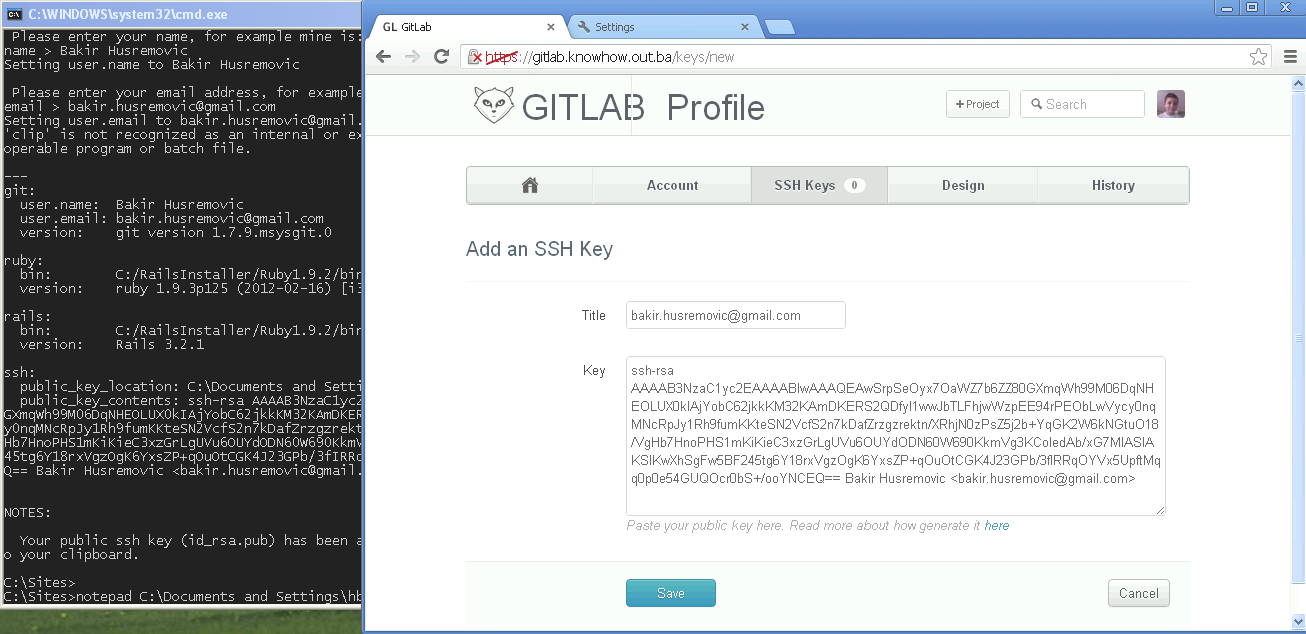
\includegraphics[width=15cm]{img/gitlab_ssh_profile.png}
\caption{Gitlab ssh profil}
\end{figure}

\section{Git workflow}

\subsection{Novi projekat}

Kreirajmo naš ''helo\_ruby'' projekat.

\begin{figure}[H]
\centering
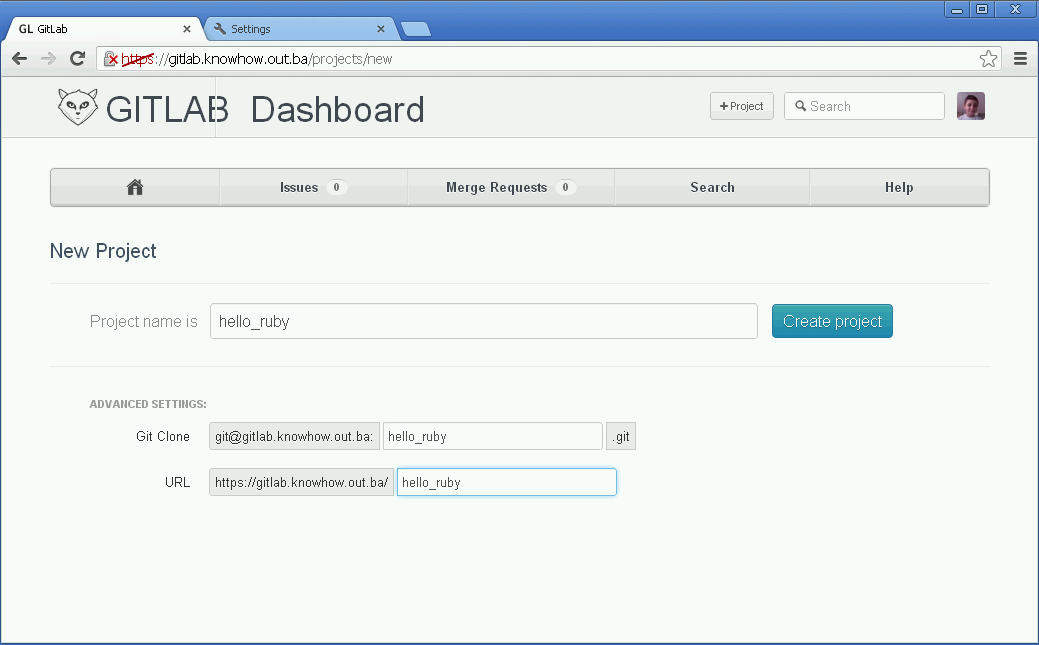
\includegraphics[width=15cm]{img/gitlab_new_project.png}
\caption{Gitlab: novi projekat}
\end{figure}


\begin{figure}[H]
\centering
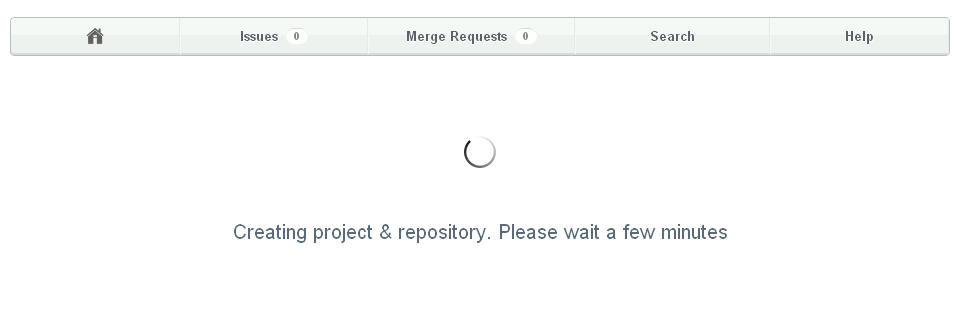
\includegraphics[width=15cm]{img/gitlab_new_project_2.png}
\caption{Gitlab: novi projekat /2}
\end{figure}


\begin{figure}[H]
\centering
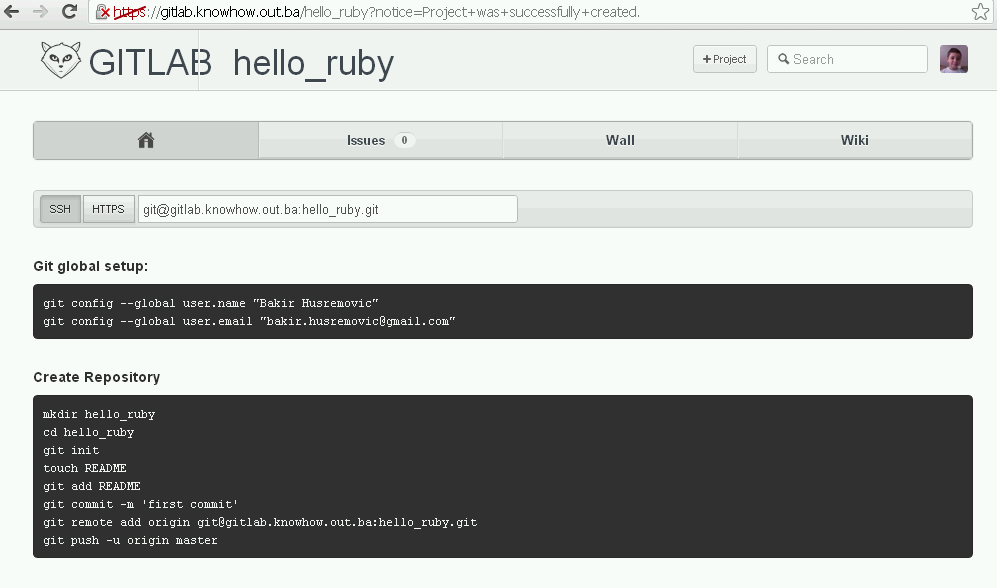
\includegraphics[width=15cm]{img/gitlab_new_project_3.png}
\caption{Gitlab: novi projekat /3}
\end{figure}


\begin{figure}[H]
\centering
\includegraphics[width=15cm]{img/gitlab_show_project.png}
\caption{Gitlab: prikaz aktivnosti za projekat}
\end{figure}



\begin{figure}[H]
\centering
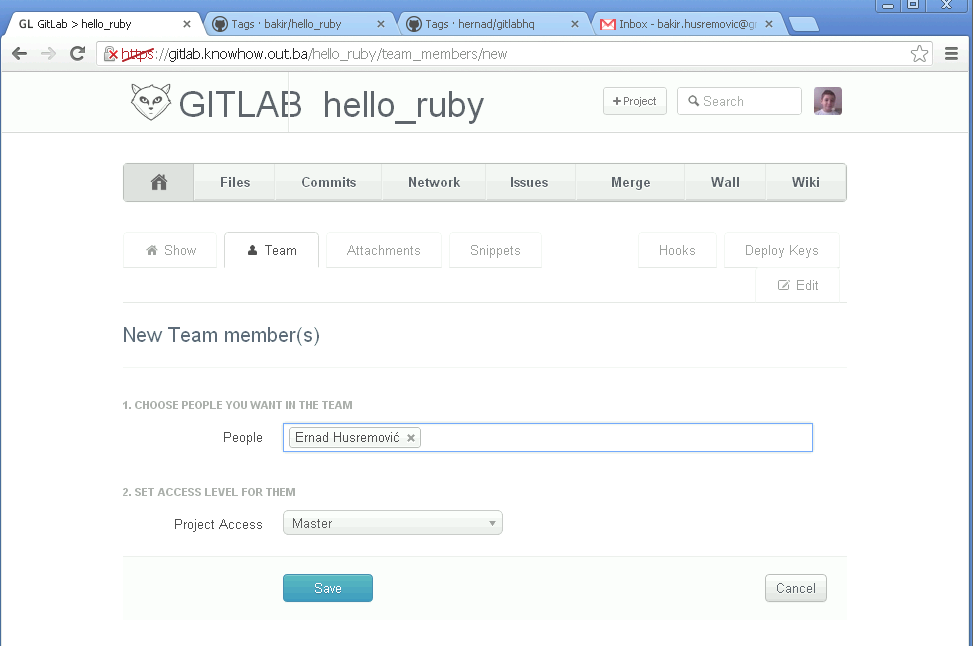
\includegraphics[width=15cm]{img/gitlab_add_new_member_to_project.png}
\caption{Gitlab: dodaj novog člana u projekat}
\end{figure}

\begin{figure}[H]
\centering
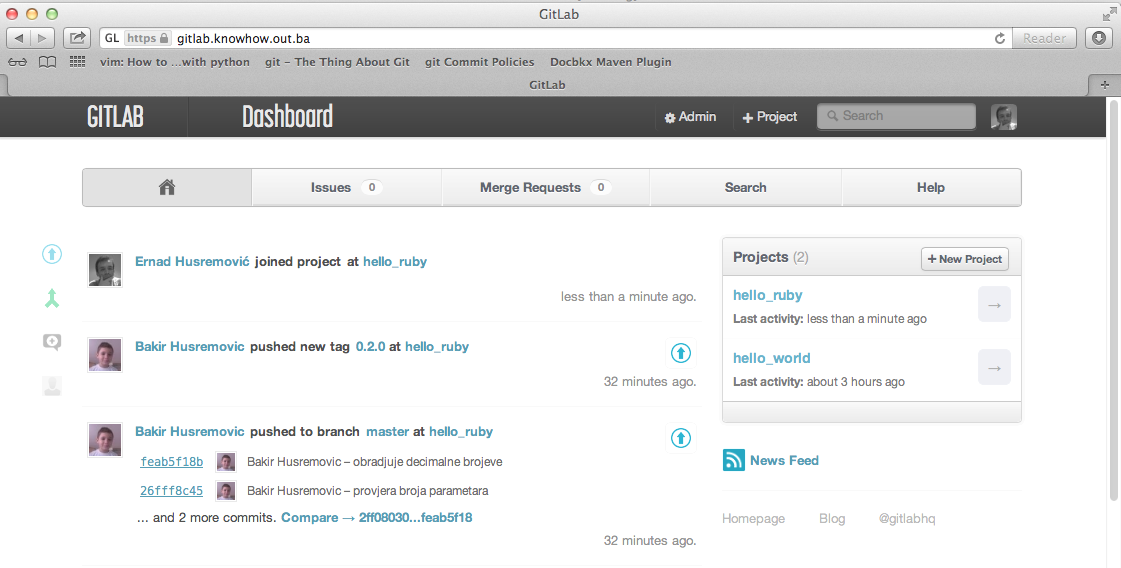
\includegraphics[width=15cm]{img/gitlab_add_new_member_to_project_2.png}
\caption{Gitlab dodaj novog člana u projekat 2}
\end{figure}




\section{Github servis}

\begin{figure}[H]
\centering
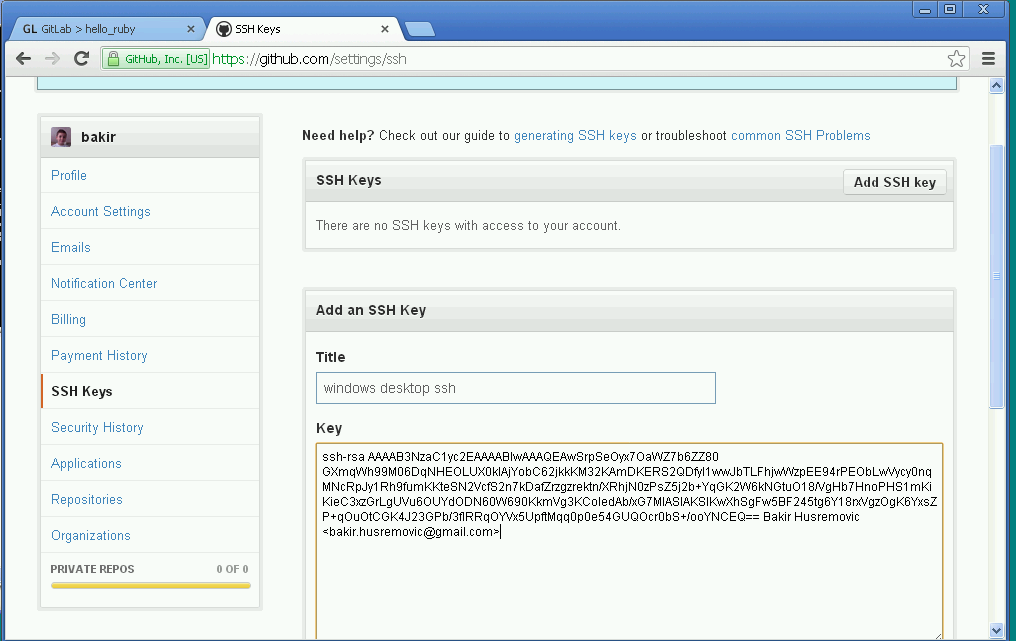
\includegraphics[width=15cm]{img/github_ssh_profile.png}
\caption{Github ssh profil}
\end{figure}

\begin{figure}[H]
\centering
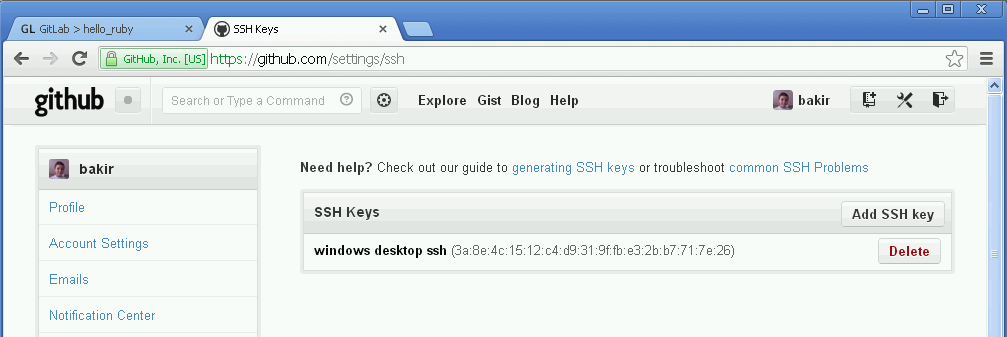
\includegraphics[width=15cm]{img/github_ssh_profile_2.png}
\caption{Github ssh profil /2}
\end{figure}


\begin{figure}[H]
\centering
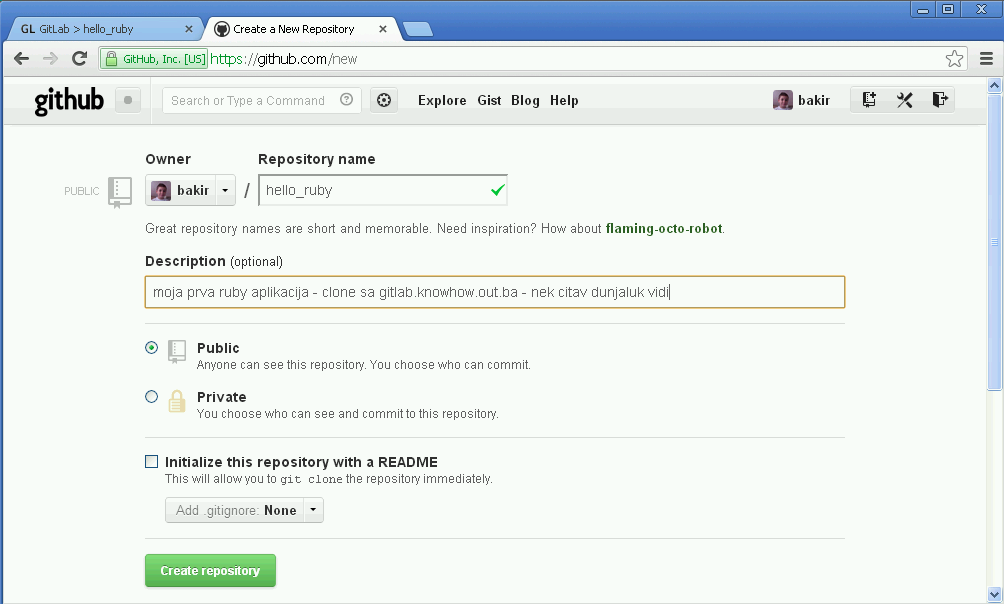
\includegraphics[width=15cm]{img/github_new_repos.png}
\caption{Github novi repozitorij}
\end{figure}

\begin{figure}[H]
\centering
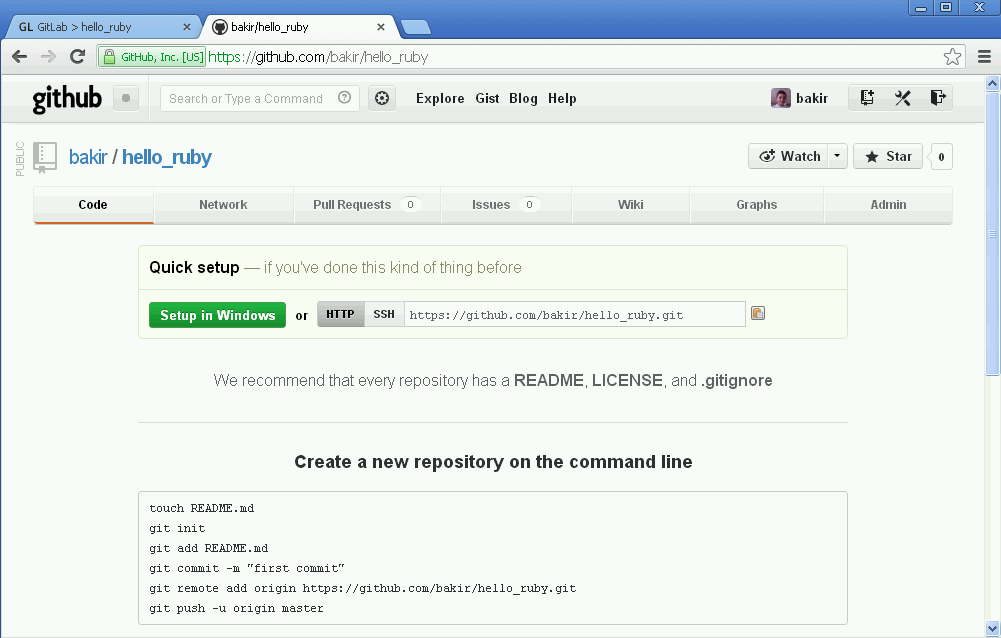
\includegraphics[width=15cm]{img/github_new_repos_2.png}
\caption{Github novi repozitorij / 2}
\end{figure}


\begin{figure}[H]
\centering
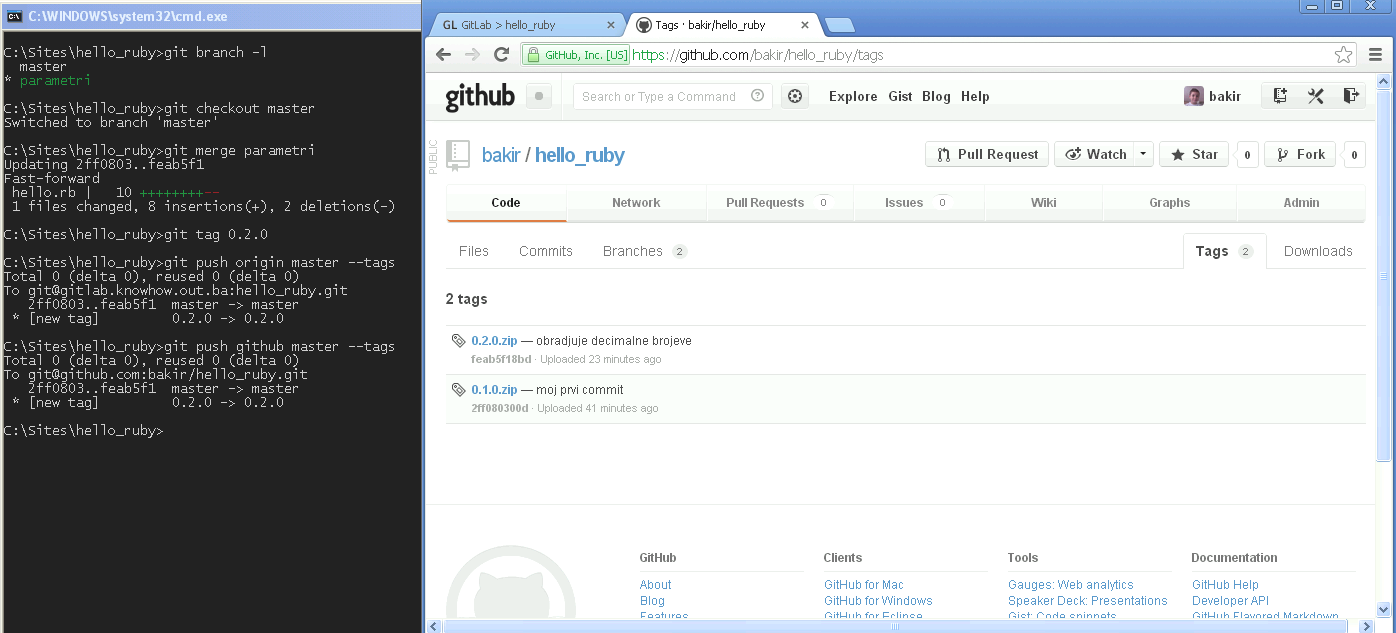
\includegraphics[width=16cm]{img/github_new_tag.png}
\caption{Github - novi tag}
\end{figure}

\begin{figure}[H]
\centering
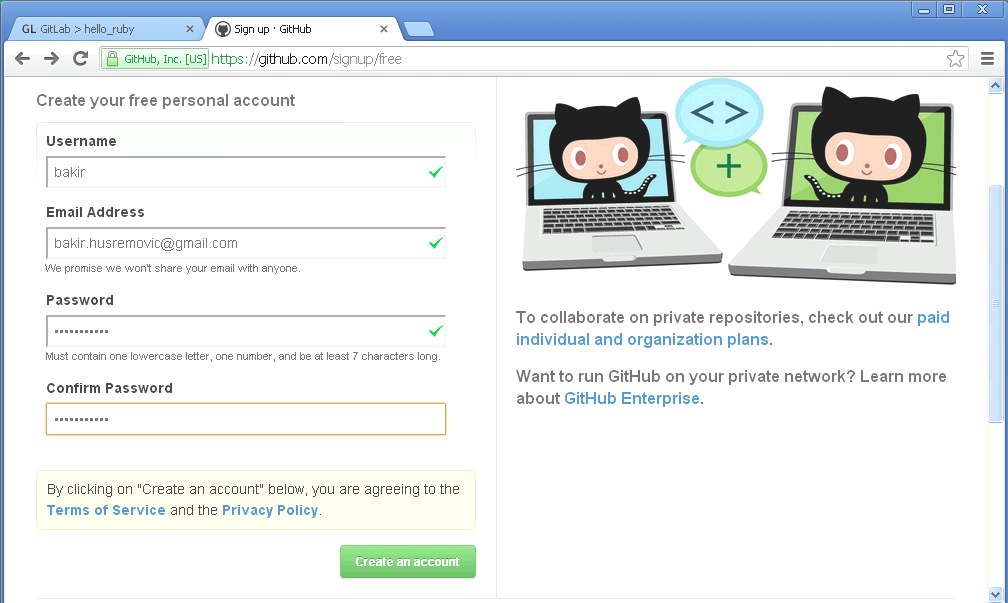
\includegraphics[width=15cm]{img/github_prijava.png}
\caption{Github prijava}
\end{figure}

\begin{figure}[H]
\centering
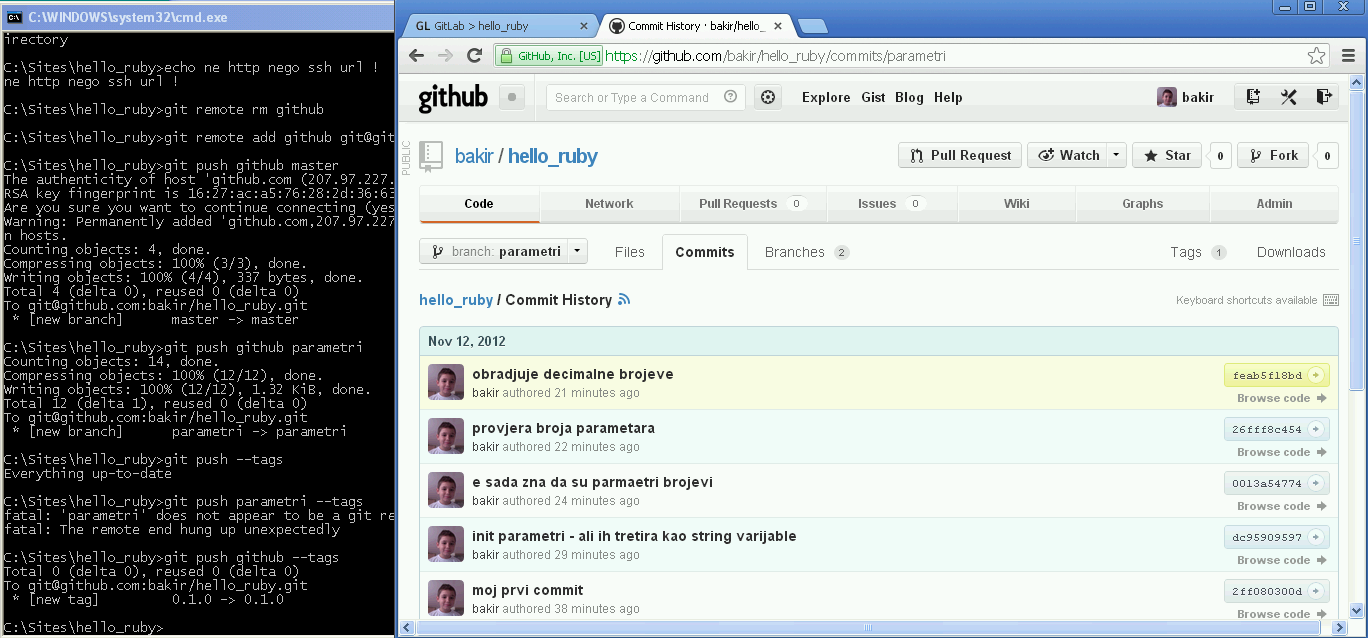
\includegraphics[width=15cm]{img/github_push_branches_and_tags.png}
\caption{Pošalji sve branchove i tag-ove na github repozitorij}
\end{figure}



\begin{figure}[H]
\centering
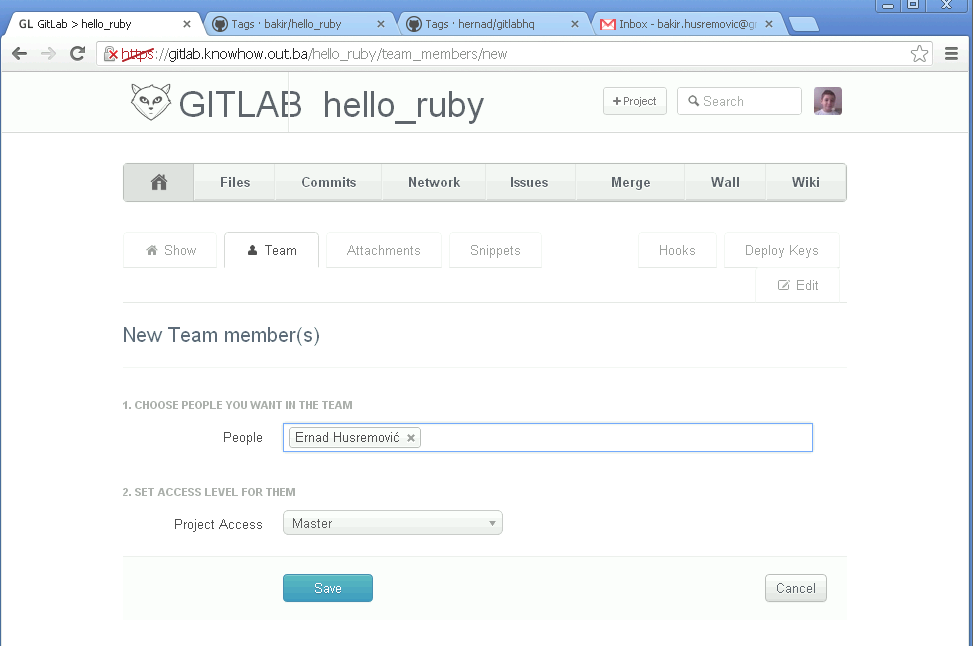
\includegraphics[width=15cm]{img/gitlab_add_new_member_to_project.png}
\caption{Gitlab: dodaj novog člana u projekat}
\end{figure}


\begin{figure}[H]
\centering
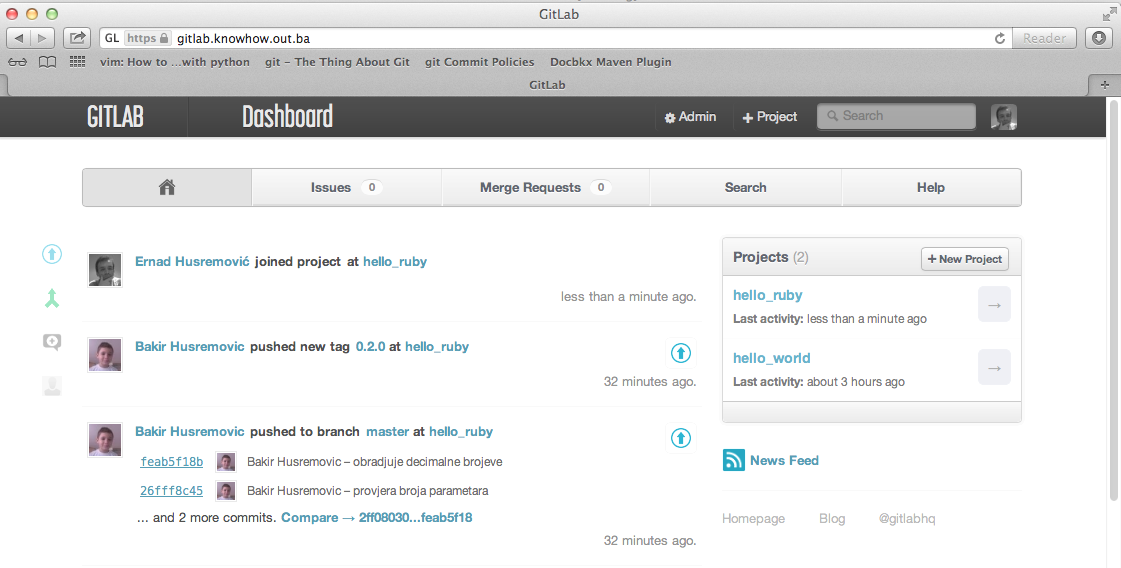
\includegraphics[width=15cm]{img/gitlab_add_new_member_to_project_2.png}
\caption{Gitlab dodaj novog člana u projekat 2}
\end{figure}


\section{Compare}

\begin{figure}[H]
\centering
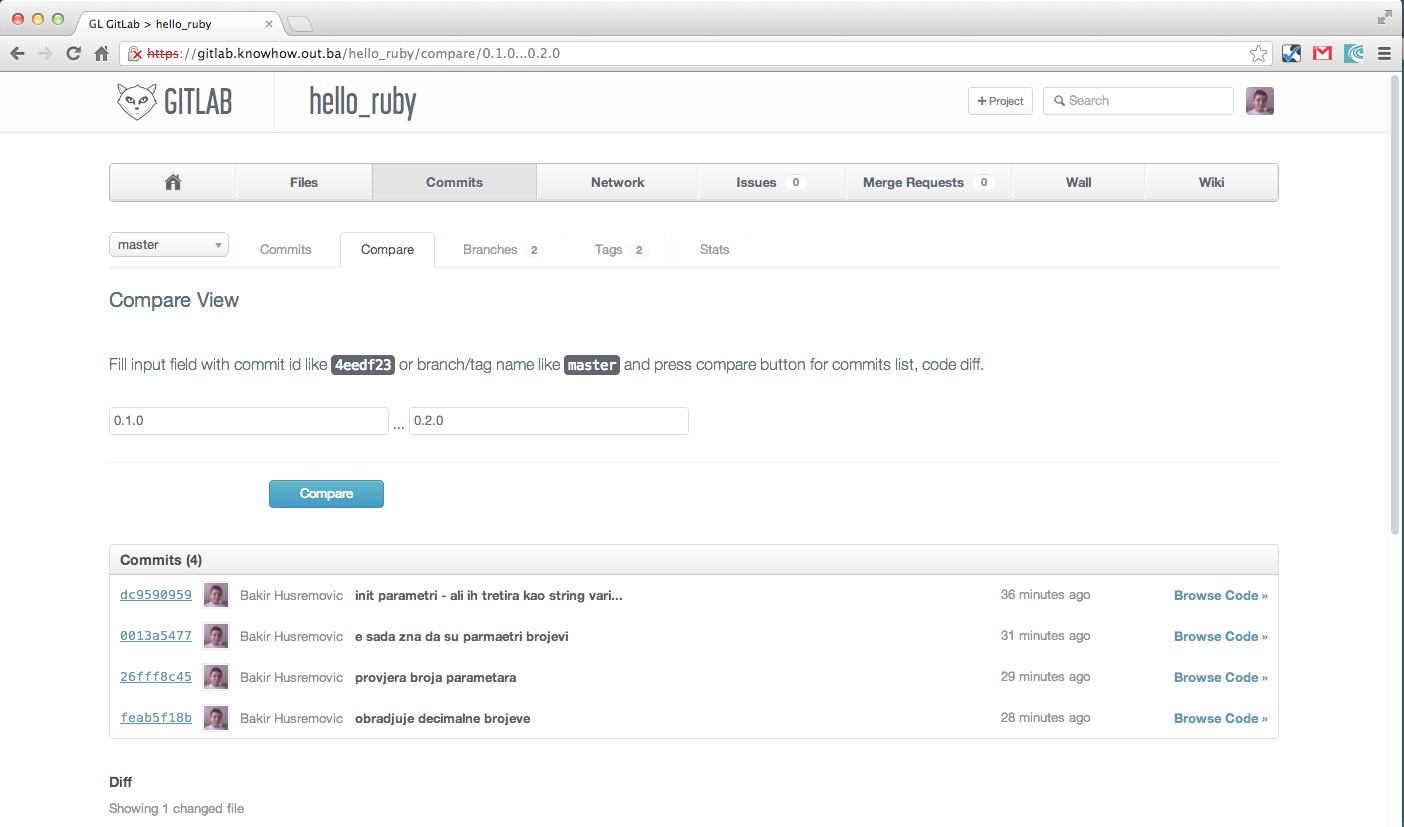
\includegraphics[width=15cm]{img/gitlab_compare.png}
\caption{Gitlab uporedi dvije verzije}
\end{figure}


\begin{figure}[H]
\centering
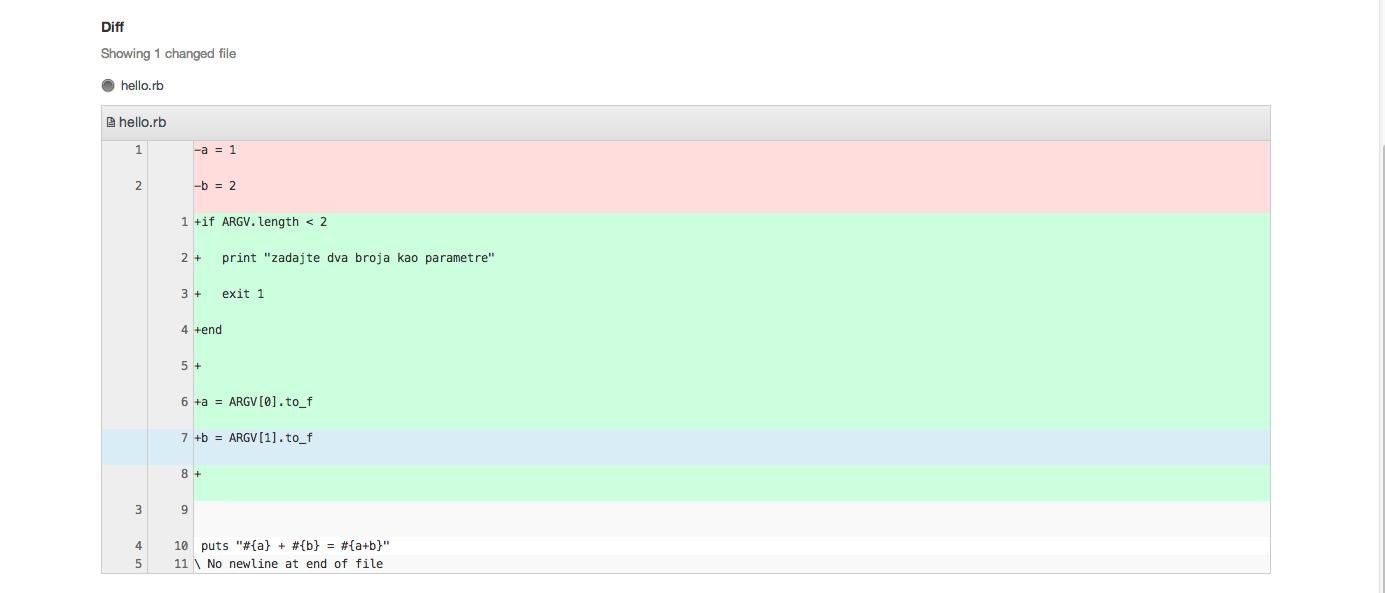
\includegraphics[width=15cm]{img/gitlab_compare_2.png}
\caption{Gitlab uporedi dvije verzije /2}
\end{figure}


\section{Notifikacija}

\begin{figure}[H]
\centering
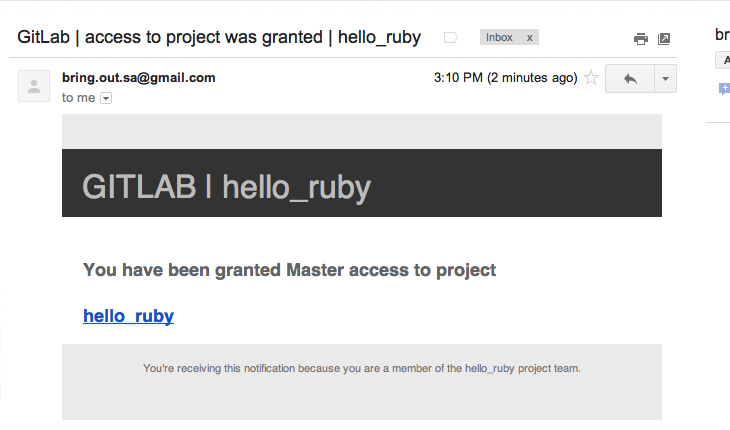
\includegraphics[width=15cm]{img/gitlab_email_notification.png}
\caption{Gitlab email notifikacija}
\end{figure}


\begin{figure}[H]
\centering
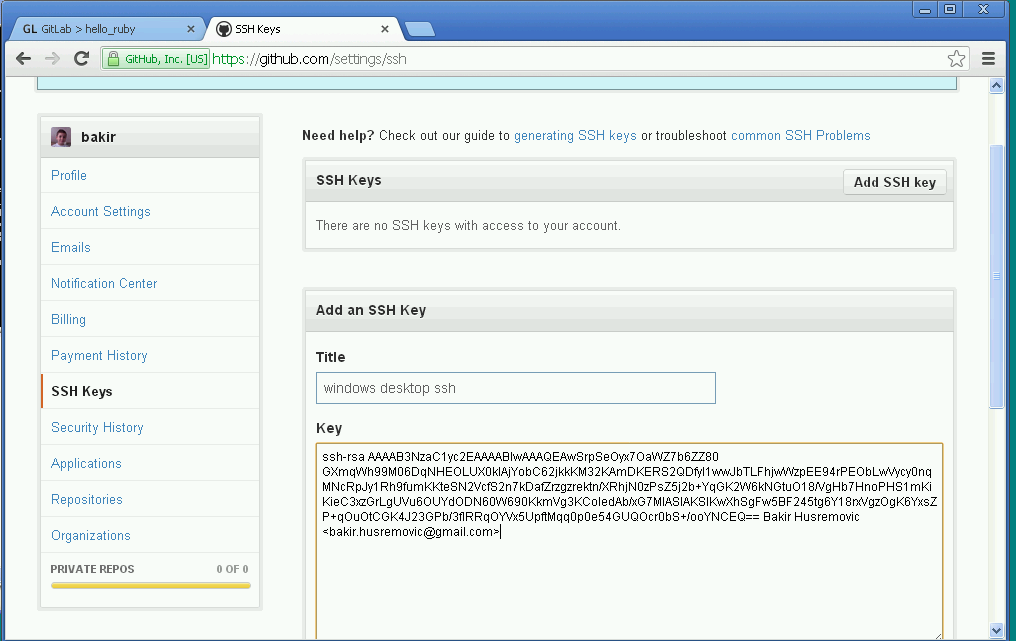
\includegraphics[width=15cm]{img/github_ssh_profile.png}
\caption{Github ssh profil}
\end{figure}



\begin{figure}[H]
\centering
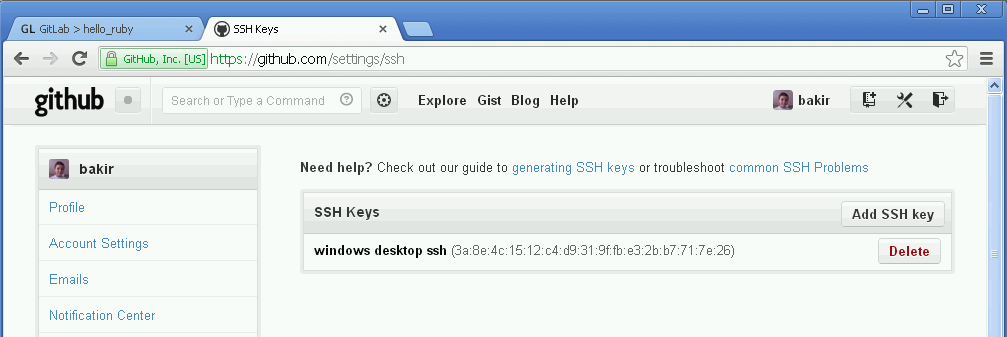
\includegraphics[width=15cm]{img/github_ssh_profile_2.png}
\caption{Github ssh profil /2}
\end{figure}

\begin{figure}[H]
\centering
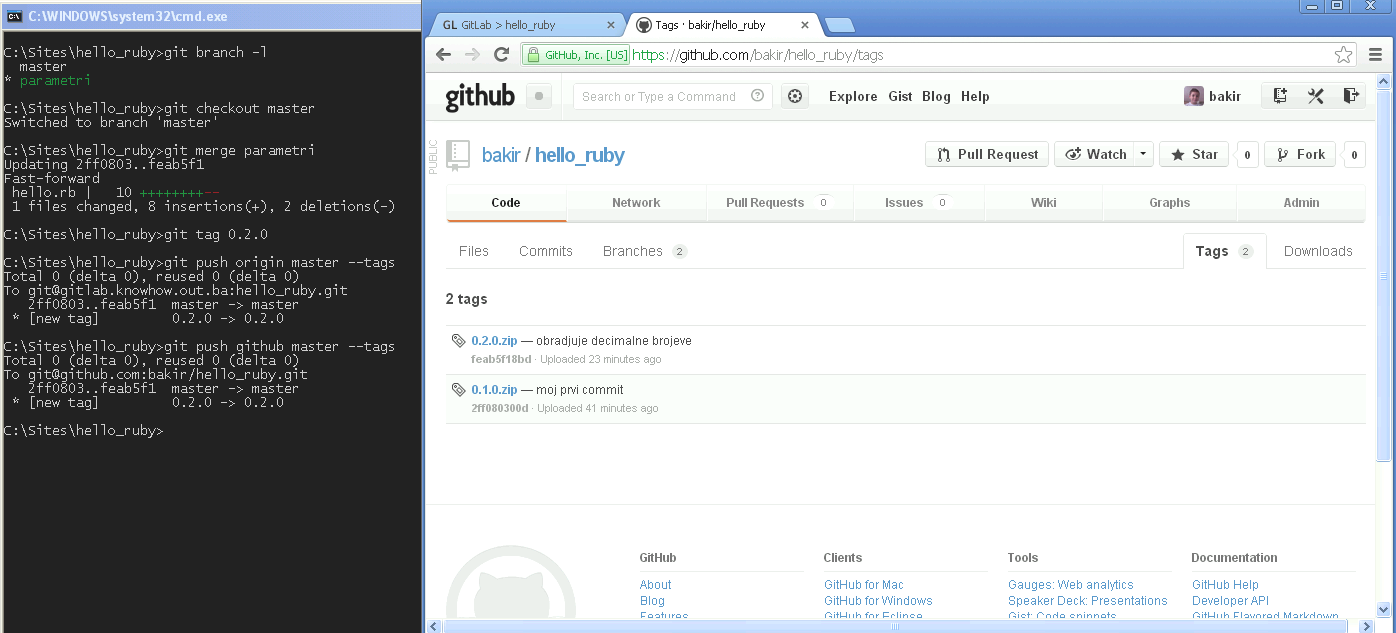
\includegraphics[width=16cm]{img/github_new_tag.png}
\caption{Github - novi tag}
\end{figure}

\begin{figure}[H]
\centering
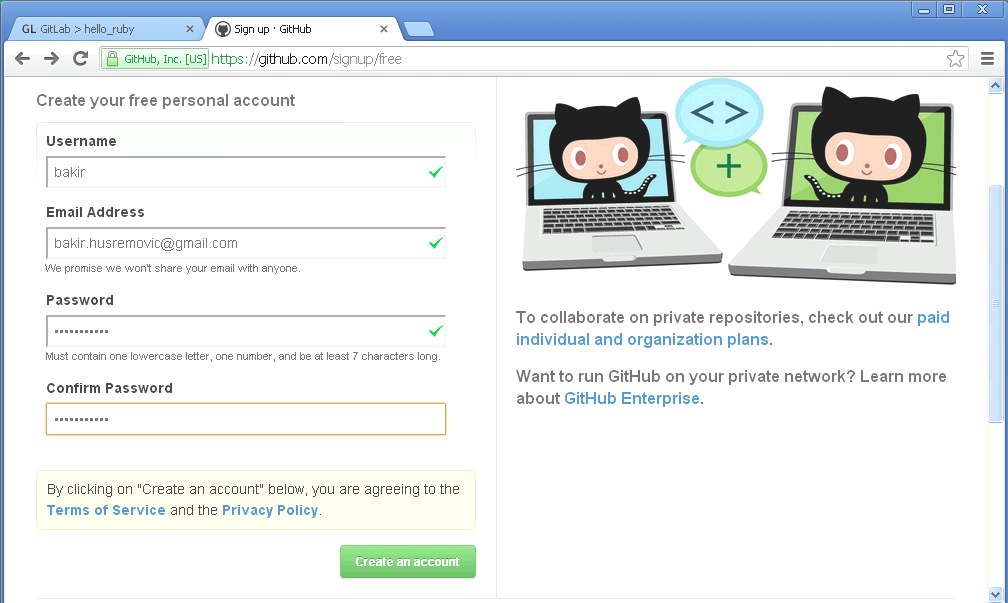
\includegraphics[width=15cm]{img/github_prijava.png}
\caption{Github prijava}
\end{figure}



%\begin{center}
%\emph{\large{Freedom to create, distribute, and use open source software (OSS).}}
%\end{center}

\chapter {Gitlab}
\vspace*{-0.7cm}

\section{Source control}

\section{Issues}

\section{Wiki}

\chapter{Zaključak}

.

% -------------------------------------------------
\bibliography{literatura}
\bibliographystyle{fit}

% -------------------------------------------------
\appendix

\chapter{Instalacija}
\vspace*{-0.7cm}
\setlength{\parindent}{0cm}
%\setlength{\parindent}{default}

\chapter{Software toolset}
\begin{enumerate}
  \item Mac OS X 10.8.2
  \item mvim, vim tekst editor ver 7.3
  \item MacTex (TeX Live 2012)
\end{enumerate}

\chapter{Software repozitoriji}

\begin{itemize}
  \item Agilni developerski environment  \url{https://github.com/hernad/atile\_dev\_env}

\end{itemize}

\end{document}
